\documentclass{article}

\usepackage{graphicx}
\usepackage{tikz}
\usepackage{tikzsymbols}
\usetikzlibrary{calc,patterns,shapes.geometric}
\pagestyle{empty}
\usepackage[margin=0pt]{geometry}
\geometry{papersize={14in,12in}}

\def\centerarc[#1](#2)(#3:#4:#5){\draw[#1] ($(#2)+({#5*cos(#3)},{#5*sin(#3)})$) arc (#3:#4:#5);}

\begin{document}
	\begin{figure}
		\centering
		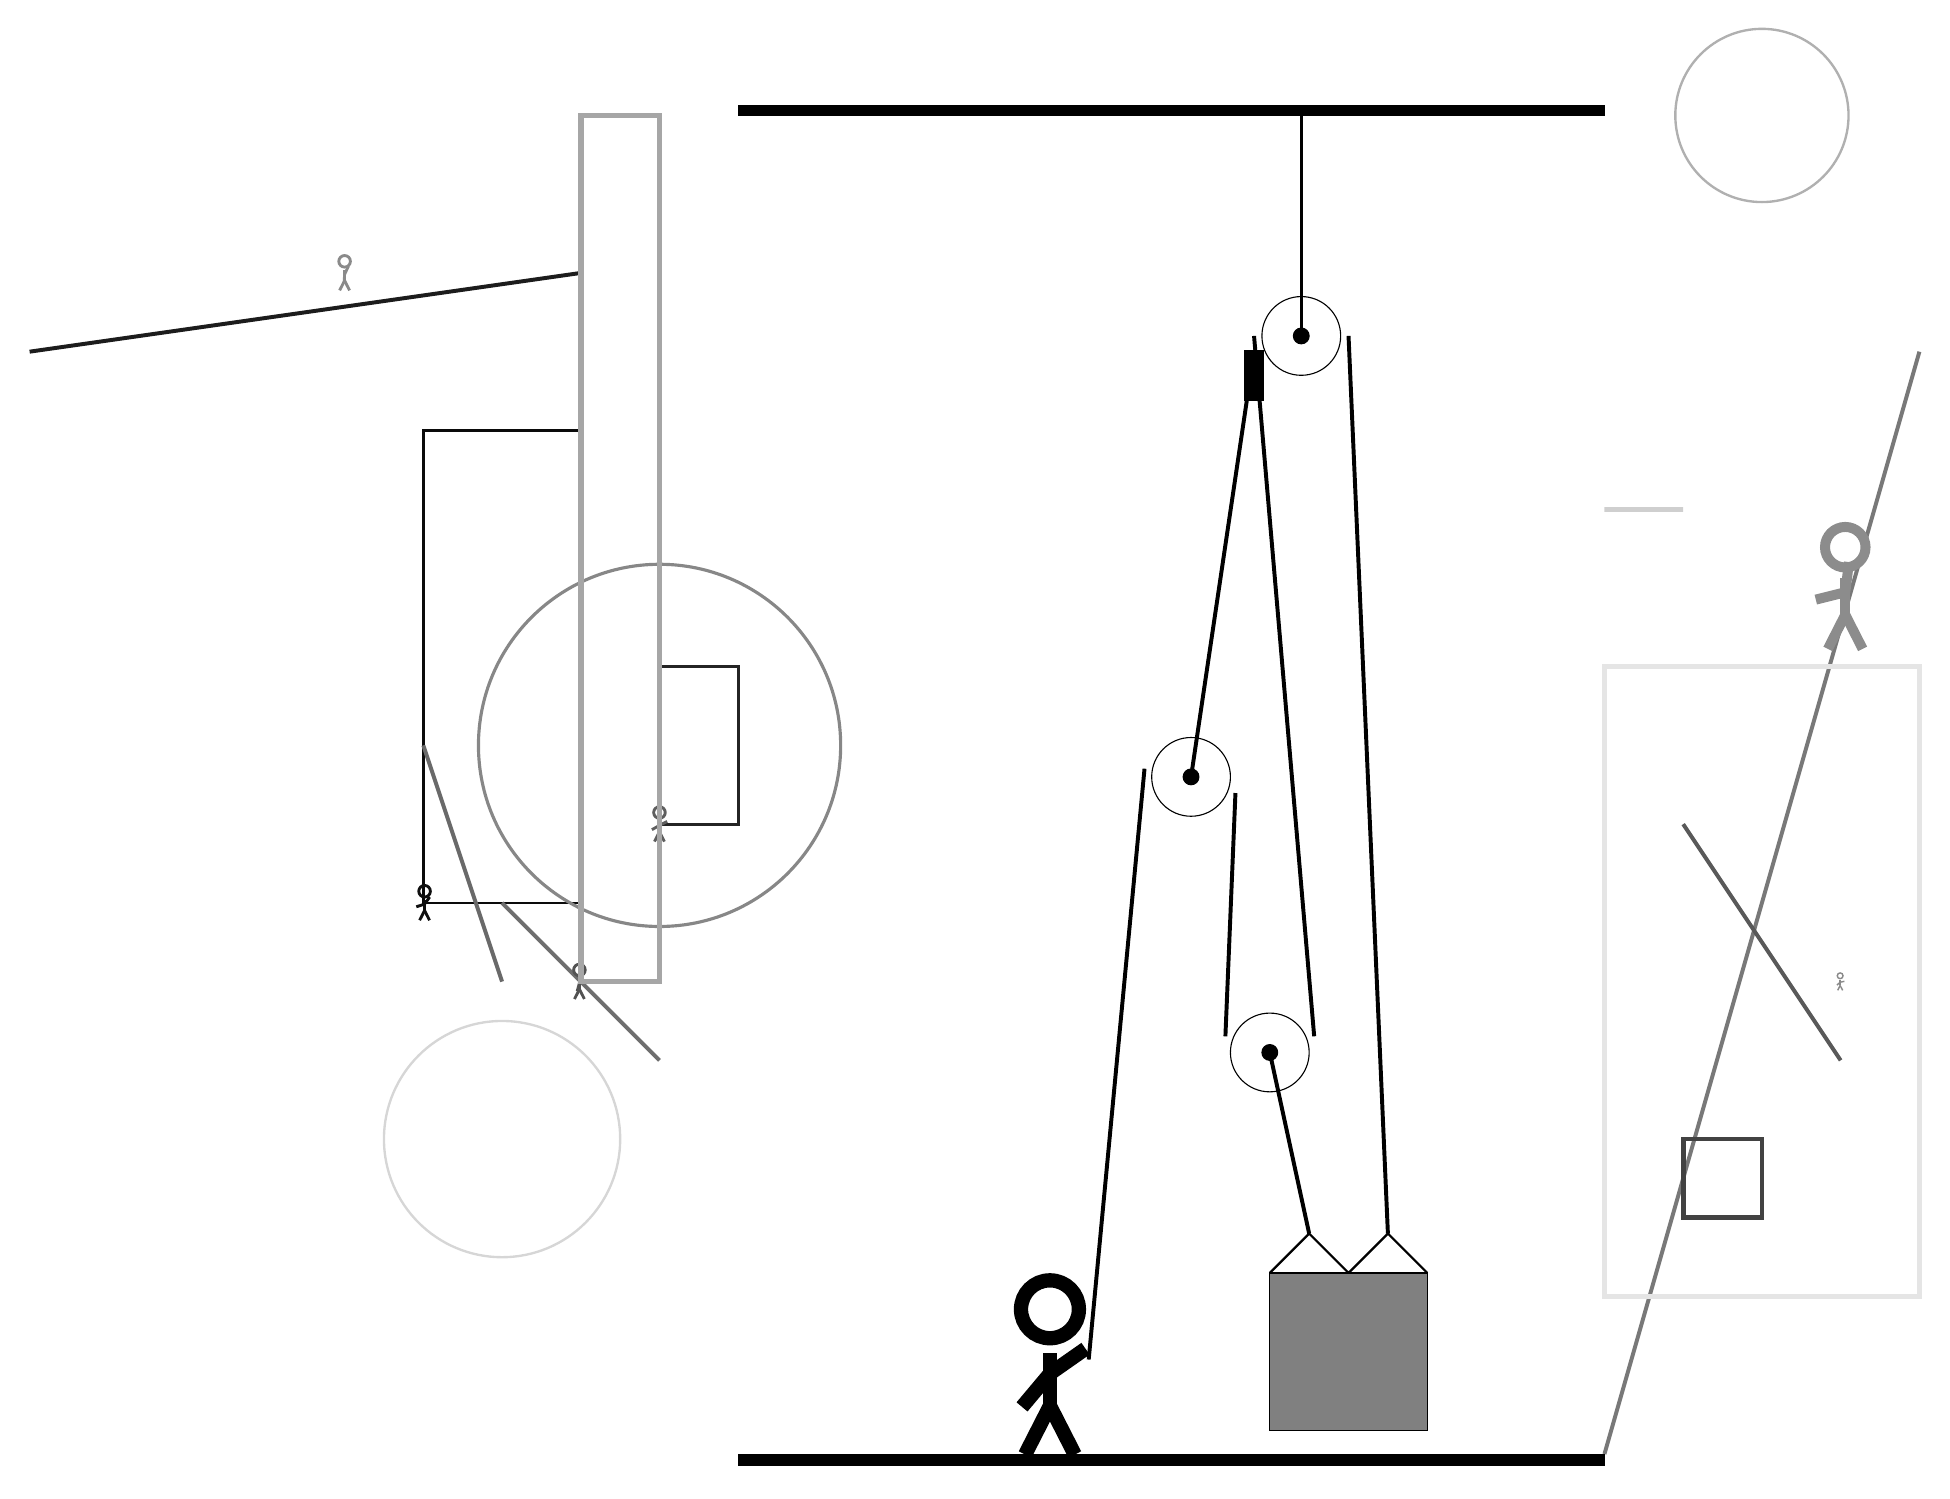
\begin{tikzpicture}
			%%%%% START %%%%%
			
			\draw[fill=black] (-6, 14) rectangle (5, 14.125);
			
			\draw (-0.25, 5.6) circle (0.5);
			\draw[fill=black] (-0.25, 5.6) circle (0.1);
			
			\draw (0.75, 2.1) circle (0.5);
			\draw[fill=black] (0.75, 2.1) circle (0.1);
			
			\draw (1.15, 11.2) circle (0.5);
			\draw[fill=black] (1.15, 11.2) circle (0.1);
			\draw[very thick] (1.15, 11.2) -- (1.15, 14);
			
			\draw[thick]  (0.75, -0.7) -- (1.25, -0.2) -- (1.75, -0.7) -- (2.25, -0.2) -- (2.75, -0.7);
			\draw[fill=black!50] (0.75, -0.7) rectangle (2.75, -2.7);
			
			\draw[line width=0.5mm] (-0.25, 5.6) -- (0.55, 11.0);
			\draw[line width=0.5mm, fill=black](0.45, 10.4) rectangle (0.65, 11.0);
			\draw[line width=0.5mm] (-1.55, -1.8) -- (-0.8409, 5.7042);
			\centerarc[line width=0.5mm](-0.25, 5.6)(-20:170:0.6);
			\draw[line width=0.5mm] (0.3138, 5.3948) -- (0.1862, 2.3052);
			\centerarc[line width=0.5mm](0.75, 2.1)(160:380:0.6);
			\draw[line width=0.5mm] (1.3138, 2.3052) -- (0.55, 11.2);
			\draw[line width=0.5mm](0.75, 2.1) -- (1.25, -0.2);
			\centerarc[line width=0.5mm](1.15, 11.2)(0:180:0.6);
			\draw[line width=0.5mm] (1.75, 11.2) -- (2.25, -0.2);
			
			\node at (-2, -1.9) {\Strichmaxerl[10][50][35]};
			
			\draw [line width=0.3mm, color=black!16](-9, 1) circle (1.5);
			
			\draw[line width=0.5mm, color=black!53](9, 11) -- (5, -3);
			\draw[line width=0.5mm, color=black!65](6, 5) -- (8, 2);
			\draw[line width=0.7mm, color=black!10] (5, -1) rectangle (9, 7);
			\draw[line width=0.6mm, color=black!19] (5, 9) rectangle (6, 9);
			\node[line width=0.3mm, color=black!46] at (-11, 12) {\Strichmaxerl[2][87][64]};
			\node[line width=0.5mm, color=black!45] at (8, 8) {\Strichmaxerl[7][14][83]};
			
			\node[line width=0.5mm, color=black!46] at (8, 3) {\Strichmaxerl[1][42][12]};
			\draw[line width=0.3mm, color=black!96] (-8, 4) rectangle (-10, 10);
			\draw[line width=0.5mm, color=black!57](-7, 2) -- (-9, 4);
			\draw[line width=0.6mm, color=black!74] (7, 1) rectangle (6, 0);
			\draw [line width=0.3mm, color=black!31](7, 14) circle (1.1);
			\draw[line width=0.4mm, color=black!86] (-7, 5) rectangle (-6, 7);
			
			\draw[line width=0.5mm, color=black!89](-8, 12) -- (-15, 11);
			\node[line width=0.4mm, color=black!94] at (-10, 4) {\Strichmaxerl[2][18][54]};
			\node[line width=0.6mm, color=black!68] at (-8, 3) {\Strichmaxerl[2][75][10]};
			
			\draw [line width=0.4mm, color=black!47](-7, 6) circle (2.3);
			\node[line width=0.4mm, color=black!63] at (-7, 5) {\Strichmaxerl[2][30][27]};
			\draw[line width=0.5mm, color=black!59](-9, 3) -- (-10, 6);
			
			\draw[line width=0.7mm, color=black!35] (-7, 3) rectangle (-8, 14);
			
			\draw[fill=black] (-6, -3) rectangle (5, -3.15);
			
			%%%%% END %%%%%
		\end{tikzpicture}
	\end{figure}	
\end{document}